\title{Introductory Electricity, Magnetism, and Optics Practice Problems}
\author{Cyrus Vandrevala}

\documentclass[11pt]{article}
\usepackage{amsmath}
\usepackage[margin=2.5cm]{geometry}
\usepackage[pdftex]{graphicx}

\begin{document}

\maketitle
\tableofcontents
\vspace{50pt}

\subsection*{Useful Constants}
Electron Mass = $9.11 \times 10^{-31}$ kg \\*
Proton Mass = $1.67 \times 10^{-27}$ kg \\*
Elementary Charge = $1.602 \times 10^{-19}$ C \\*
Coulomb's Constant = $8.99 \times 10^9$ Nm$^2$/C$^2$ \\*
Permittivity of Free Space = $8.85 \times 10^{-12} s^4 A^2 / (kg \cdot s^4)$ \\*
Permeability of Free Space = $1.25 \times 10^{-6} m \cdot kg / (s^2 A^2)$ \\*
Speed of Light in a Vacuum = $3 \times 10^8$ m/s \\*
Acceleration Due to Gravity = 9.81 m/s$^2$

%%%%%%%%%%%%%%%%%%%%%%%%%%%%%%%%%%%%%%%%%%%%%%%%%%%%%%%%%%%%%%%%%%%%%%%%%%%%%%

\pagebreak
\section{AC Circuits}
\vspace{10pt}

\subsection{Resonant Frequency of Series RLC Circuit}
A series RLC circuit contains a resistor (R = 200 $\Omega$), a capacitor (C = 2.00 $\mu$F), an inductor (L = 2.00 H), and a battery with some voltage V.  The amplitude of the current going through the circuit is I = 1.00 A.  Determine the resonant frequency of the circuit. \\* \\*
$\Rightarrow $ 500 rad/s

\subsection{RMS Power in a Series RLC Circuit}
A series RLC circuit contains a resistor (R = 200 $\Omega$), a capacitor (C = 2.00 $\mu$F), an inductor (L = 2.00 H), and a battery with some voltage V.  The amplitude of the current going through the circuit is I = 1.00 A.  Determine the RMS power going through the resistor. \\* \\*
$\Rightarrow $ 100 W


%%%%%%%%%%%%%%%%%%%%%%%%%%%%%%%%%%%%%%%%%%%%%%%%%%%%%%%%%%%%%%%%%%%%%%%%%%%%%%

\pagebreak
\section{Properties of Light}
\vspace{10pt}

\subsection{Time of Travel}
A beam of light travels through 10 m of plastic with an index of refraction of n = 1.50; a second beam of light travels through 13 m of vacuum.  Which beam of light will complete its journey in a shorter amount of time? \\* \\*
$\Rightarrow$ The one travelling through vacuum.

\subsection{Plane Electromagnetic Wave Equation \#1}
A plane electromagnetic wave is propagating in the +z direction in free space.  The instantaneous electric field vector is given by:
\begin{equation}
\vec{E}(x,y,z,t) = E_o \hspace{0.01cm}cos(kz - \omega t) \hat{i}
\end{equation}
What is the amplitude of the magnetic field associated with the wave?\\* \\*
$\Rightarrow |\vec{B}| = E_o / c$

\subsection{Plane Electromagnetic Wave Equation \#2}
A plane electromagnetic wave is propagating in the +z direction in free space.  The instantaneous electric field vector is given by:
\begin{equation}
\vec{E}(x,y,z,t) = E_o \hspace{0.01cm}cos(kz - \omega t) \hat{i}
\end{equation} 
Write out the equation for the magnetic field of the electromagnetic wave.\\* \\*
$\Rightarrow \vec{B}(x,y,z,t) = \frac{E_o}{c} \hspace{0.01cm}cos(kz - \omega t) \hat{j}$

\pagebreak
\subsection{Radiation Pressure}
A laser beam of power 5.60 W and diameter 1.30 mm is directed upward at one circular face of a perfectly reflecting cylinder, which is made to "hover" by the beam's radiation pressure.  Each face of the cylinder has an area A = 100 mm$^2$.  The cylinder has a density of 1200 kg/m$^3$.  What is the height (H) of the cylinder?  You may assume that the cylinder is completely contained within the laser beam.

\begin{center}
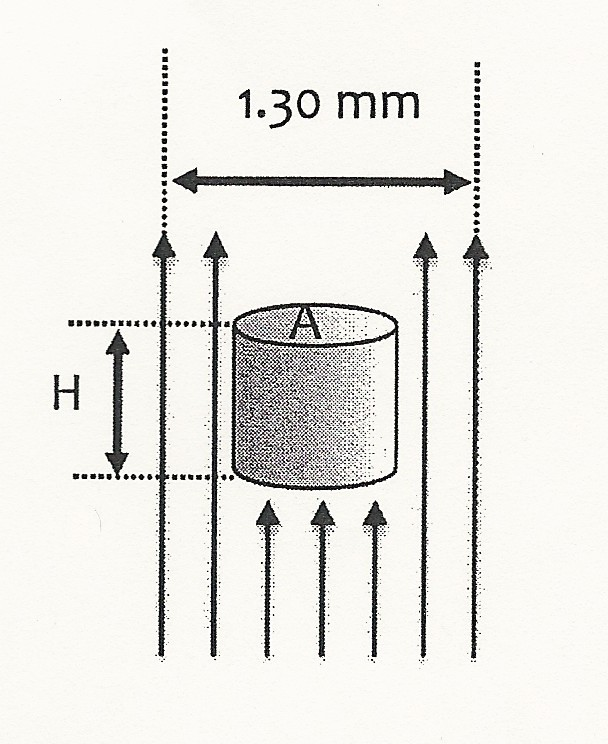
\includegraphics[scale=0.2]{Images/radiation_pressure.jpg}
\end{center}

$\Rightarrow$ H = 1.2 $\mu$m

%%%%%%%%%%%%%%%%%%%%%%%%%%%%%%%%%%%%%%%%%%%%%%%%%%%%%%%%%%%%%%%%%%%%%%%%%%%%%%

\pagebreak
\section{Polarizing Filters}
\vspace{10pt}

\subsection{Maximum Intensity}
I shine unpolarized light on two polarizing filters are oriented $90^\circ$ with respect to each other.  I place a third polarizing filter in between the two.  At what angle should I insert the third polarizing filter such that it lets as much light through the system as possible? \\* \\*
$\Rightarrow 45^\circ$ with respect to the first polarizer

\subsection{Exchanging Polarizers}
Suppose I have a system of three polarizers oriented as such:
\begin{itemize}
\item[1.] Polarizer \#1 oriented at $10^\circ$ with respect to the horizontal.
\item[2.] Polarizer \#2 oriented at $20^\circ$ with respect to the horizontal.
\item[3.] Polarizer \#3 oriented at $30^\circ$ with respect to the horizontal.
\end{itemize}
I shine initially unpolarized light on the system, and it exits with some intensity $I_{final}$.  If I were to swap polarizer \#2 and polarizer \#3, how would the intensity change? \\* \\*
$\Rightarrow$ It would stay the same.

%%%%%%%%%%%%%%%%%%%%%%%%%%%%%%%%%%%%%%%%%%%%%%%%%%%%%%%%%%%%%%%%%%%%%%%%%%%%%%

\pagebreak
\section{Geometric Optics}
\vspace{10pt}

\subsection{Refraction \#1}
I shine a laser beam from the bottom of a pool of water as shown below.  What is the maximum angle $\theta$ the laser can make with the vertical and still emerge into the air above the plastic?

\begin{center}
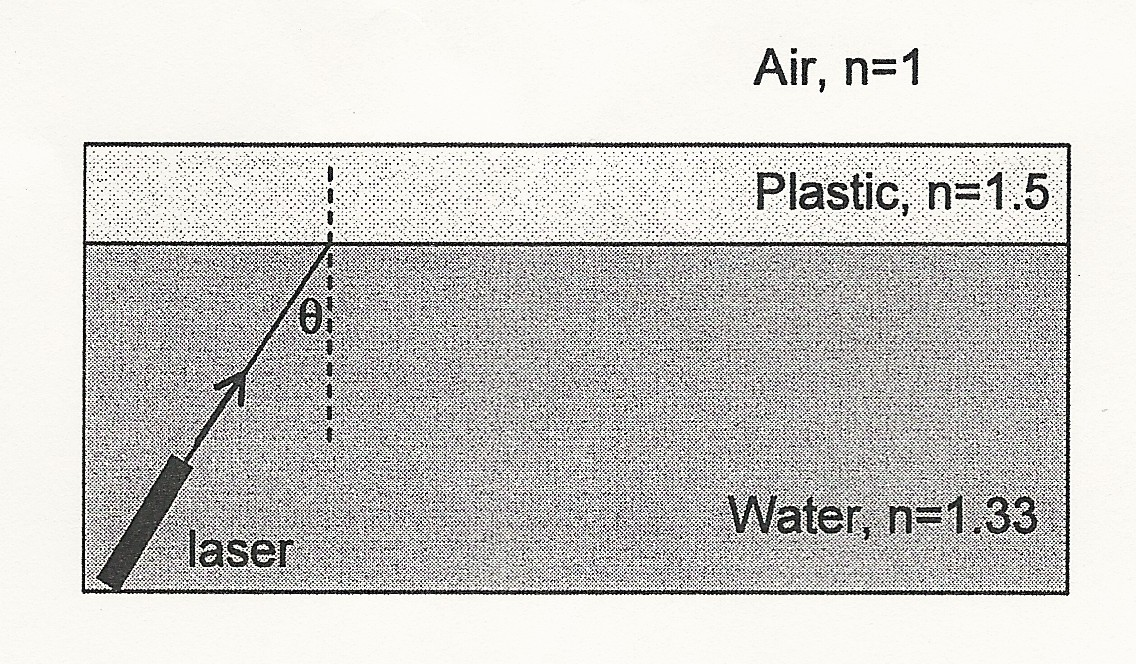
\includegraphics[scale=0.2]{Images/slab_of_water_and_plastic.jpg}
\end{center}

$\Rightarrow 48.75^\circ$

%%%%%%%%%%%%%%%%%%%%%%%%%%%%%%%%%%%%%%%%%%%%%%%%%%%%%%%%%%%%%%%%%%%%%%%%%%%%%%%

\end{document}